% \iffalse meta-comment
% (The MIT License)
%
% Copyright (c) 2021-2025 Yegor Bugayenko
%
% Permission is hereby granted, free of charge, to any person obtaining a copy
% of this software and associated documentation files (the 'Software'), to deal
% in the Software without restriction, including without limitation the rights
% to use, copy, modify, merge, publish, distribute, sublicense, and/or sell
% copies of the Software, and to permit persons to whom the Software is
% furnished to do so, subject to the following conditions:
%
% The above copyright notice and this permission notice shall be included in all
% copies or substantial portions of the Software.
%
% THE SOFTWARE IS PROVIDED 'AS IS', WITHOUT WARRANTY OF ANY KIND, EXPRESS OR
% IMPLIED, INCLUDING BUT NOT LIMITED TO THE WARRANTIES OF MERCHANTABILITY,
% FITNESS FOR A PARTICULAR PURPOSE AND NONINFRINGEMENT. IN NO EVENT SHALL THE
% AUTHORS OR COPYRIGHT HOLDERS BE LIABLE FOR ANY CLAIM, DAMAGES OR OTHER
% LIABILITY, WHETHER IN AN ACTION OF CONTRACT, TORT OR OTHERWISE, ARISING FROM,
% OUT OF OR IN CONNECTION WITH THE SOFTWARE OR THE USE OR OTHER DEALINGS IN THE
% SOFTWARE.
% \fi

%%% \CheckSum{0}
%
% \CharacterTable
%  {Upper-case    \A\B\C\D\E\F\G\H\I\J\K\L\M\N\O\P\Q\R\S\T\U\V\W\X\Y\Z
%   Lower-case    \a\b\c\d\e\f\g\h\i\j\k\l\m\n\o\p\q\r\s\t\u\v\w\x\y\z
%   Digits        \0\1\2\3\4\5\6\7\8\9
%   Exclamation   \!     Double quote  \"     Hash (number) \#
%   Dollar        \$     Percent       \%     Ampersand     \&
%   Acute accent  \'     Left paren    \(     Right paren   \)
%   Asterisk      \*     Plus          \+     Comma         \,
%   Minus         \-     Point         \.     Solidus       \/
%   Colon         \:     Semicolon     \;     Less than     \<
%   Equals        \=     Greater than  \>     Question mark \?
%   Commercial at \@     Left bracket  \[     Backslash     \\
%   Right bracket \]     Circumflex    \^     Underscore    \_
%   Grave accent  \`     Left brace    \{     Vertical bar  \|
%   Right brace   \}     Tilde         \~}

% \GetFileInfo{yb-book.dtx}
% \DoNotIndex{\end,\empty,\defined,\def,\begin,\if,\isempty,\endgroup,\begingroup,\let,\else,\fi,\newcommand,\newenvironment}

% \iffalse
%<*driver>
\ProvidesFile{yb-book.dtx}
%</driver>
%<class>\NeedsTeXFormat{LaTeX2e}
%<class>\ProvidesClass{yb-book}
%<*class>
[0000/00/00 0.0.0 YB Branded Book Style]
%</class>
%<*driver>
\documentclass{ltxdoc}
\usepackage[tt=false, type1=true]{libertine}
\usepackage{microtype}
\AddToHook{env/verbatim/begin}{\microtypesetup{protrusion=false}}
\usepackage{href-ul}
\usepackage{graphicx}
\PageIndex
\EnableCrossrefs
\CodelineIndex
\RecordChanges
\begin{document}
	\DocInput{yb-book.dtx}
	\PrintChanges
	\PrintIndex
\end{document}
%</driver>
% \fi

% \title{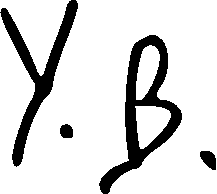
\includegraphics[width=0.75in]{yb-book-logo.pdf} \\ \LaTeX{} Class |yb-book|\thanks{The sources are in GitHub at \href{https://github.com/yegor256/yb-book.cls}{yegor256/yb-book.cls}}}
% \author{Yegor Bugayenko \\ \texttt{yegor256@gmail.com}}
% \date{\filedate, \fileversion}
%
% \maketitle
%
% \section{Introduction}
%
% \index{Amazon}
% The provided class |yb-book| helps me design
% \href{https://www.yegor256.com/books.html}{my books} and
% publish them
% \href{https://www.amazon.com/Yegor-Bugayenko/e/B01AM1QMDK}{on Amazon}.
% You are welcome to use is for your own books. It is as simple
% as this:
%\iffalse
%<*verb>
%\fi
\begin{verbatim}
\documentclass{yb-book}
\renewcommand*\thetitle{New Book About OOP}
\renewcommand*\theauthor{Jeff Lebowski}
\renewcommand*\thevolume{1}
\renewcommand*\theversion{1.0}
\begin{document}
\ybPrintTitlePage
\chapter{First One}
\section{About Something Interesting}
Hello, world!
\end{document}
\end{verbatim}
%\iffalse
%</verb>
%\fi

% You are welcome to suggest additional options and commands, but the style
% of my books is intentionally as simple as possible, avoiding formatting
% as much as possible. Here is \href{https://www.yegor256.com/2019/05/21/dont-improvise.html}{why}.

% \section{Options}

% There are a few class options you can use:

% \begin{macro}{compact}
% Use this package option when you need to make text more compact
% and take less vertical space. This may be convenient fiction books.
% I use this option to render \href{https://www.yegor256.com/code-ahead.html}{Code Ahead} book.
% \end{macro}

% \begin{macro}{sparse}
% With this package option every section will start from a new page.
% \end{macro}

% \begin{macro}{manuscript}
% When the format is not for Amazon printing,
% but for some other purposes (the page size is A4), this option may be
% convenient. I also use it when I want the book to be rendered for
% printing on paper for review purposes.
% \end{macro}

% \begin{macro}{authordraft}
% \changes{v0.4.0}{2024/03/23}{The package option \texttt{draft} renamed to \texttt{draft}}
% When it's a draft for reviewers (the page size is A4)
% and you want to have a watermark and a compact form of the content. This
% option goes together with |\thereviewer{}| command, which you may redefine,
% in order to embed the name of the reviewed in the watermark. This may
% help you prevent theft of your book:
%\iffalse
%<*verb>
%\fi
\begin{verbatim}
\documentclass[authordraft]{yb-book}
\renewcommand*\thereviewer{Walter Sobchak}
\begin{document}
Hello, world!
\end{document}
\end{verbatim}
%\iffalse
%</verb>
%\fi
% \end{macro}

% \section{Meta Commands}

% There are a number of commands that you may redefine in the preamble:
%\iffalse
%<*verb>
%\fi
\begin{verbatim}
\documentclass{yb-book}
\newcommand*\thetitle{My New Book About OOP}
\newcommand*\theauthor{Yegor Bugayenko}
\newcommand*\thevolume{1}
\newcommand*\thedate{24 Feb 2022}
\newcommand*\theversion{1.4}
\newcommand*\thereviewer{Jeff Lebowski}
\begin{document}
... the content goes here ...
\end{document}
\end{verbatim}
%\iffalse
%</verb>
%\fi

% \section{Printers}

% There are a number of printers --- commands that print large blocks of text
% in the expected format:

% \begin{macro}{\ybPrintTitlePage}
% Prints the first page of a book. It expects at least |\thetitle|
% and |theauthor| to be defined:
%\iffalse
%<*verb>
%\fi
\begin{verbatim}
\documentclass{yb-book}
\renewcommand*\thetitle{My New Book}
\renewcommand*\theauthor{Yegor Bugayenko}
\begin{document}
\ybPrintTitlePage
.. the rest of the book goes here
\end{document}
\end{verbatim}
%\iffalse
%</verb>
%\fi
% \end{macro}

% \begin{macro}{\ybPrintTOC}
% Prints the table of contents.
% \end{macro}

% \begin{macro}{\ybQuote}
% Prints a side quote:
%\iffalse
%<*verb>
%\fi
\begin{verbatim}
\documentclass{yb-book}
\begin{document}
Hello, world!
\ybQuote{Never tell the truth to people who
  are not worthy of it}{Mark Twain}{}
\end{document}
\end{verbatim}
%\iffalse
%</verb>
%\fi
% \end{macro}

% \begin{macro}{\ybPrintBibliography}
% Prints the list of bib references.
% \end{macro}

% \begin{macro}{\ybPrintIndex}
% Prints index with an optional name of the section (instead of ``Index''):
%\iffalse
%<*verb>
%\fi
\begin{verbatim}
\documentclass{yb-book}
\begin{document}
Hello, world!
\ybPrintIndex{Recommended Books}
\end{document}
\end{verbatim}
%\iffalse
%</verb>
%\fi
% \end{macro}

% \StopEventually{}

% \section{Implementation}

% \changes{v0.1.0}{2022/01/09}{Initial version}
% \changes{v0.2.0}{2022/10/02}{Started using l3build}

% First, we parse package options:
% \changes{v0.3.0}{2023/05/22}{The \texttt{pgfopts} package is now used to parse package options.}
% \changes{v0.5.0}{2024/01/02}{The \texttt{sparse} package option added, to place every section in a new page.}
% \changes{v0.6.0}{2025/01/08}{The \texttt{apa} package option added, to enable APA citation style.}
%    \begin{macrocode}
\RequirePackage{pgfopts}
\pgfkeys{
  /yb/.cd,
  apa/.store in=\yb@apa,
  authordraft/.store in=\yb@authordraft,
  compact/.store in=\yb@compact,
  manuscript/.store in=\yb@manuscript,
  sparse/.store in=\yb@sparse,
}
\ProcessPgfPackageOptions{/yb}
%    \end{macrocode}

% Then, depending on the options like |authordraft| and |manuscript|, we preset
% options of the class |book| and then load it:
%    \begin{macrocode}
\makeatletter
\ifdefined\yb@authordraft
  \PassOptionsToClass{11pt}{book}
  \PassOptionsToClass{oneside}{book}
\else
  \ifdefined\yb@manuscript
    \PassOptionsToClass{12pt}{book}
    \PassOptionsToClass{oneside}{book}
  \else
    \PassOptionsToClass{11pt}{book}
    \PassOptionsToClass{twoside}{book}
  \fi
\fi
\makeatother
\LoadClass{book}
%    \end{macrocode}

% Then, we load \href{https://ctan.org/pkg/inputenc}{inputenc} for UTF-8 encoding of the sources:
% \changes{v0.5.1}{2025/01/05}{Added the usage of \texttt{inputenc} in order to ensure UTF-8 encoding for the sources.}
%    \begin{macrocode}
\RequirePackage[utf8]{inputenc}
%    \end{macrocode}

% \begin{macro}{geometry}
% Then, using |geometry|, we setup page layout:
%    \begin{macrocode}
\RequirePackage{geometry}
\geometry{
  paperwidth=6in, paperheight=9in,
  bindingoffset=0.25in,
  left=0.75in, right=0.75in, top=0.75in, bottom=1.25in}
\makeatletter
\ifdefined\yb@authordraft
  \geometry{a4paper, margin=1in, left=1.5in}
\else
  \ifdefined\yb@manuscript
    \geometry{a4paper, margin=1.2in}
  \fi
\fi
\makeatother
%    \end{macrocode}
% \end{macro}

% Then, we load \href{https://ctan.org/pkg/href-ul}{href-ul} to underline links correctly:
%    \begin{macrocode}
\RequirePackage{href-ul}
%    \end{macrocode}

% Then, we load \href{https://ctan.org/pkg/anyfontsize}{anyfontsize} to enable all sizes of fonts:
%    \begin{macrocode}
\RequirePackage{anyfontsize}
%    \end{macrocode}

% Then, we load \href{https://ctan.org/pkg/tikz}{tikz} for graphics:
%    \begin{macrocode}
\RequirePackage{tikz}
  \usetikzlibrary{positioning}
  \usetikzlibrary{shapes}
  \usetikzlibrary{fit}
%    \end{macrocode}

% Then, we load \href{https://ctan.org/pkg/chngcntr}{chngcntr} for something else:
%    \begin{macrocode}
\RequirePackage{chngcntr}
  \counterwithout{footnote}{chapter}
%    \end{macrocode}

% Then, we load \href{https://ctan.org/pkg/lastpage}{lastpage} to enable rendering of the last page number:
%    \begin{macrocode}
\RequirePackage{lastpage}
%    \end{macrocode}

% Then, we load \href{https://ctan.org/pkg/paralist}{paralist} for inline enumeration:
%    \begin{macrocode}
\RequirePackage{paralist}
%    \end{macrocode}

% Then, we load \href{https://ctan.org/pkg/xcolor}{xcolor} for colors:
%    \begin{macrocode}
\RequirePackage{xcolor}
%    \end{macrocode}

% Then, we load \href{https://ctan.org/pkg/graphicx}{graphicx} to enable graphic files inclusion:
%    \begin{macrocode}
\RequirePackage{graphicx}
%    \end{macrocode}

% Then, we load \href{https://ctan.org/pkg/enumitem}{enumitem} for inline enumeration:
%    \begin{macrocode}
\RequirePackage[inline]{enumitem}
  \setlist{nosep}
%    \end{macrocode}

% Then, we load \href{https://ctan.org/pkg/float}{float} for floating figures:
%    \begin{macrocode}
\RequirePackage{float}
%    \end{macrocode}

% Then, we load \href{https://ctan.org/pkg/ulem}{ulem} for inline lists:
%    \begin{macrocode}
\RequirePackage[normalem]{ulem}
%    \end{macrocode}

% Then, we load \href{https://ctan.org/pkg/xfp}{xfp} and
% \href{https://ctan.org/pkg/xifthen}{xifthen} for if-then-else:
%    \begin{macrocode}
\RequirePackage{xfp}
\RequirePackage{xifthen}
%    \end{macrocode}

% Then, we load \href{https://ctan.org/pkg/soul}{soul} for highlighting:
%    \begin{macrocode}
\RequirePackage{soul}
%    \end{macrocode}

% Then, we load \href{https://ctan.org/pkg/csquotes}{csquotes} for better rendering:
%    \begin{macrocode}
\RequirePackage[autostyle=try]{csquotes}
%    \end{macrocode}

% \begin{macro}{\pagestyle}
% Then, we set the layout of a page to |plain|:
%    \begin{macrocode}
\pagestyle{plain}
%    \end{macrocode}
% \end{macro}

% \begin{macro}{setspace}
% Then, using |setspace| package we set the spacing between lines in the text,
% depending on the package options:
%    \begin{macrocode}
\RequirePackage{setspace}
  \setstretch{1.2}
  \makeatletter
  \ifdefined\yb@compact\setstretch{1.0}\fi
  \ifdefined\yb@manuscript\setstretch{1.1}\fi
  \ifdefined\yb@authordraft\setstretch{1.5}\fi
  \makeatother
%    \end{macrocode}
% \end{macro}

% \begin{macro}{biblatex}
% Then, we configure |biblatex|, for citation management:
%    \begin{macrocode}
\PassOptionsToPackage{indexing=cite,
  natbib=true,maxnames=2,minnames=1,doi=true,
  url=false,isbn=false,isbn=false}{biblatex}
\makeatletter
\ifdefined\yb@apa
  \PassOptionsToPackage{style=authoryear}{biblatex}
\else
  \PassOptionsToPackage{style=numeric}{biblatex}
\fi
\makeatother
\RequirePackage{doi}
\RequirePackage{biblatex}
  \DeclareCiteCommand{\citetitle}
    {\boolfalse{citetracker}%
     \boolfalse{pagetracker}%
     \usebibmacro{prenote}}
    {\ifciteindex
       {\indexnames{labelname}}
       {}%
     \printfield[citetitle]{labeltitle}}
    {\multicitedelim}
    {\usebibmacro{postnote}}
  \DeclareCiteCommand*{\citetitle}
    {\boolfalse{citetracker}%
     \boolfalse{pagetracker}%
     \usebibmacro{prenote}}
    {\ifciteindex
       {\indexnames{labelname}}
       {}%
     \printfield[citetitle]{title}}
    {\multicitedelim}
    {\usebibmacro{postnote}}
%    \end{macrocode}
% \end{macro}

% \begin{macro}{condensed}
% Then, we define |condensed| environment for snippets
% (|lsstyle| is defined by |letterspace| in |microtype|):
%    \begin{macrocode}
\newenvironment{condensed}
  {\begingroup\setstretch{1.0}\lsstyle}
  {\endgroup}
%    \end{macrocode}
% \end{macro}

% \begin{macro}{microtype}
% Then, we include |microtype| for better rendering:
%    \begin{macrocode}
\makeatletter
\ifdefined\yb@authordraft\else
  \PassOptionsToPackage{letterspace=-50,nopatch=footnote}{microtype}
  \RequirePackage{microtype}
\fi
\makeatother
%    \end{macrocode}
% \end{macro}

% \begin{macro}{libertine}
% Then, we include |libertine|, for a good looking font:
%    \begin{macrocode}
\makeatletter
\ifdefined\yb@manuscript
  \RequirePackage[tt=false,type1=true]{libertine}
\fi
\makeatother
%    \end{macrocode}
% \end{macro}

% \begin{macro}{\section}
% Then, we redefine |\section| command:
%    \begin{macrocode}
\makeatletter
\let\yb@oldsection\section
\def\yb@secstart{\ifdefined\yb@sparse\newpage\fi}
\ifdefined\yb@authordraft
  \RequirePackage[medium]{titlesec}
\else
  \RequirePackage[raggedright]{titlesec}
    \titlespacing{\section}{0in}{6pt}{6pt}[1in]
  \renewcommand\section{\yb@secstart\yb@oldsection}
\fi
\ifdefined\yb@compact
  \renewcommand\section{\yb@secstart\vspace{2em}\yb@oldsection}
\fi
\makeatother
%    \end{macrocode}
% \end{macro}

% Then, if it's a |authordraft|, we put a watermark comment:
%    \begin{macrocode}
\makeatletter
\ifdefined\yb@authordraft
  \RequirePackage[absolute]{textpos}
    \TPGrid{16}{16}
  \RequirePackage{fancyhdr}
  \pagestyle{fancy}
  \renewcommand\headrulewidth{0pt}
  \renewcommand\footrulewidth{0pt}
  \setlength{\headheight}{16pt}
  \fancyhf{}
  \fancyhead[L,C,LO,CO]{}
  \fancyhead[R,RO]{
    \begin{textblock}{16}[0.5,0.5](8,8)%
      \tikz \node[minimum width=16\TPHorizModule] {%
        \fontsize{64}{64}\selectfont\bfseries%
        \rotatebox{45}{
          \tikz \node
          [fill=gray!6, font=\ttfamily\color{white}]
          {it is a draft};%
        }%
      };%
    \end{textblock}%
    \begin{textblock}{4}(11.5,1)%
      \tikz \node [color=gray, rotate=270,
        font=\ttfamily\scriptsize, text width=8in] at (0,0) {%
        Copyright \textcopyright{} \the\year{} by \theauthor{}.
        All rights reserved. No part of the contents of
        this book may be reproduced or transmitted in any
        form or by any means without the written permission
        of the publisher. This particular manuscript is
        printed for \textbf{\thereviewer{}} and may be used only
        for one-time review. The manuscript has to be destroyed
        after the review.%
      };
    \end{textblock}
  }
  \fancyfoot[C,CO,C]{\small\ttfamily%
    page \#\thepage{} of \pageref{LastPage}}
\fi
\makeatother
%    \end{macrocode}

% \begin{macro}{\maketitle}
% Then, we redefine |\maketitle| command:
%    \begin{macrocode}
\renewcommand\maketitle{
  {\LARGE\textbf{\thetitle}}
  \\[1em]
  by \theauthor{}
  \\[4em]
  \ifx\thevolume\empty\else%
    Volume \thevolume{}\\
  \fi
  \ifx\thedate\empty\else%
    Rendered on \thedate{}
  \fi
  \ifx\theversion\empty\else%
    \\
    Ver. \theversion{}
  \fi
}
%    \end{macrocode}
% \end{macro}

% \begin{macro}{\ybPrintTitlePage}
% Then, we define |\ybPrintTitlePage| command:
%    \begin{macrocode}
\makeatletter
\newcommand\ybPrintTitlePage{
  \ifdefined\yb@authordraft\else
    \begin{titlepage}
      \ttfamily
      \vspace*{\fill}
      \noindent
      {\Huge\thetitle}
      \\[1em]
      by \theauthor{}
      \\[4em]
      \ifx\thevolume\empty\else%
        Volume \thevolume{}\\
      \fi
      \ifx\thedate\empty\else%
        \thedate{}
      \fi
      \ifx\thedate\empty\else%
        \\
        \theversion{}
      \fi
      \vspace*{\fill}
    \end{titlepage}
  \fi
}
\makeatother
%    \end{macrocode}
% \end{macro}

% \begin{macro}{\ybPrintTOC}
% Then, we define |ybPrintTOC| command to print table of contents:
%    \begin{macrocode}
\makeatletter
\newcommand\ybPrintTOC{
  \ifdefined\yb@authordraft\else
    \ifdefined\yb@compact\else\cleardoublepage\fi
    {\setstretch{0.7}\tableofcontents}
  \fi
}
\makeatother
%    \end{macrocode}
% \end{macro}

% \begin{macro}{\ybPrintIndex}
% Then, we configure |imakeidx| package and define |\ybPrintIndex| command:
%    \begin{macrocode}
\RequirePackage{imakeidx}
  \renewbibmacro*{citeindex}{\indexnames{labelname}{}}
  \makeindex
  \indexsetup{othercode={\hyphenpenalty=10000}}
\makeatletter
\newcommand\ybPrintIndex[1][Index]{%
  \ifdefined\yb@authordraft\else
    \cleardoublepage%
    {%
      \setstretch{1.0}%
      \small%
      \addcontentsline{toc}{chapter}{#1}%
      \printindex%
    }%
  \fi%
}
\makeatother
%    \end{macrocode}
% \end{macro}

% \begin{macro}{\ybQuote}
% Then, with the help of |wrapfig| and |mdframed|, we define |\ybQuote| command:
%    \begin{macrocode}
\RequirePackage{wrapfig}
\RequirePackage{mdframed}
\RequirePackage{changepage}
  \strictpagecheck
\mdfdefinestyle{quoteodd}{backgroundcolor=black!0,
  leftmargin=6pt,rightmargin=0pt,
  innerleftmargin=6pt,innerrightmargin=0pt,
  innertopmargin=0pt,innerbottommargin=0pt,
  skipabove=0pt,skipbelow=0pt,
  linewidth=2pt,
  topline=false,bottomline=false,rightline=false}
\mdfdefinestyle{quoteeven}{backgroundcolor=black!0,
  rightmargin=6pt,leftmargin=0pt,
  innerrightmargin=6pt,innerleftmargin=0pt,
  innertopmargin=0pt,innerbottommargin=0pt,
  skipabove=0pt,skipbelow=0pt,
  linewidth=2pt,
  topline=false,bottomline=false,leftline=false}
\makeatletter
\newcommand\ybQuote[3]{%
  \ifthenelse{\isempty{#3}}{}{
    \ifx\hfuzz#2\hfuzz%
      \index{#3}%
    \else%
      \index{#3, #2}%
    \fi%
  }%
  \def\yb@body{%
    \raggedright%
    \ifx\hfuzz#3\hfuzz%
      #1%
    \else%
      ``#1''\\\raggedleft---#2 #3%
    \fi%
  }
  \ifdefined\yb@authordraft%
    \begin{wrapfigure}{r}{0.4\textwidth}%
      \begin{mdframed}[style=quoteodd]%
        \yb@body%
      \end{mdframed}%
    \end{wrapfigure}%
  \else%
    \begin{wrapfigure}{o}[12pt]{0.4\textwidth}%
      \sffamily\checkoddpage%
      \ifoddpage%
        \begin{mdframed}[style=quoteodd]\yb@body\end{mdframed}%
      \else%
        \begin{mdframed}[style=quoteeven]\yb@body\end{mdframed}%
      \fi%
      \vspace{-12pt}
    \end{wrapfigure}%
  \fi%
}
\makeatother
%    \end{macrocode}
% \end{macro}

% Then, we use and configure |footmisc| as suggested
% \href{https://tex.stackexchange.com/questions/40072/incompatibility-between-footmisc-option-multiple-and-hyperref/62091#62091}{here}:
%    \begin{macrocode}
\RequirePackage{perpage}
\RequirePackage[bottom,perpage,multiple]{footmisc}
\makeatletter
  \let\yb@oldfootnote\footnote
\newcommand\yb@nexttoken\relax
\newcommand\yb@isfootnote{%
  \ifx\footnote\yb@nexttoken\textsuperscript{,}\fi}
\renewcommand\footnote[1]{%
  \yb@oldfootnote{#1}\futurelet\yb@nexttoken\yb@isfootnote}
\makeatother
%    \end{macrocode}

% \begin{macro}{\ybPrintBibliography}
% Then, we define |\ybPrintBibliography|, to print a list of references:
% \changes{v0.6.2}{2025/01/19}{The \texttt{\char`\\ybPrintBibliography} command has an optional argument, which is the title of the chapter.}
%    \begin{macrocode}
\makeatletter
\newcommand\ybPrintBibliography[1][Bibliography]{%
  \AtNextBibliography{\small}%
  \raggedright%
  \ifdefined\yb@manuscript%
    \setlength\bibitemsep{0pt}%
    \newpage%
    \begin{multicols}{2}%
      {\setstretch{1.0}\printbibliography}%
    \end{multicols}%
  \else%
    \setlength\bibitemsep{.2em}%
    \printbibliography[heading=bibintoc,title={#1}]%
  \fi%
}
\makeatother
%    \end{macrocode}
% \end{macro}

% Then, a few layout configurations at the beginning of the document:
%    \begin{macrocode}
\AtBeginDocument{%
  \raggedbottom%
  \makeatletter
    \ifdefined\yb@authordraft
      \raggedright%
    \fi%
  \makeatother
  \setlength\topskip{0mm}%
  \setlength\parindent{0pt}%
  \setlength\fboxsep{0pt}%
  \setlength\parskip{6pt}%
  \interfootnotelinepenalty=10000%
}
%    \end{macrocode}

% Finally, a few meta commands with default values:
%    \begin{macrocode}
\newcommand*\thetitle{\textbackslash{}thetitle}
\newcommand*\thevolume{}
\newcommand*\thedate{}
\newcommand*\theversion{\textbackslash{}theversion}
\newcommand*\theauthor{\textbackslash{}theauthor}
\newcommand*\thereviewer{\textbackslash{}thereviewer}

\endinput
%    \end{macrocode}

% \Finale

%\clearpage
%
%\PrintChanges
%\clearpage
%\PrintIndex
